\documentclass{article}

%
% 引入模板的style文件
%
\usepackage{homework}

\setCJKmainfont{SimSun}[AutoFakeBold] %宋体加粗
\setCJKsansfont{SimHei}[AutoFakeBold] %黑体加粗


\usepackage{minted} %配合minted宏包进行好看的高亮
\usepackage{currfile} %配合minted宏包进行好看的高亮
\usepackage{caption} %配合minted宏包进行好看的高亮
\usepackage{tcolorbox} %配合minted宏包进行好看的高亮
\usepackage{xcolor} %配合minted宏包进行好看的高亮
\tcbuselibrary{skins} %配合minted宏包进行好看的高亮
\tcbuselibrary{minted} %配合minted宏包进行好看的高亮
\usemintedstyle{paraiso-dark} %配合minted宏包进行好看的高亮
\usepackage{framed} 
\usepackage{amsmath}


%
% 封面
%


\title{
	
\includegraphics[width=0.6\textwidth]{images/title/ucas_logo 1.pdf}\\
    \vspace{1in}
    \textmd{\textbf{\hmwkClass}}\\
	\textmd{\Large{\textbf{\hmwkClassID}}}\\
    \textmd{\textbf{\hmwkTitle}}\\
    \normalsize\vspace{0.1in}\large{\hmwkCompleteTime }\\
    \vspace{0.1in}\large{\textit{\hmwkClassInstructor\ }}\\
    \vspace{1in}
	
\includegraphics[width=0.25\textwidth]{images/title/Cyber.jpg}\\
	\vspace{1in}
}

\author{
	\hmwkAuthorName \\ 
	\hmwkAuthorStuID \\
	\hmwkAuthorInst \\
	\hmwkAuthorzhuanye \\
	\hmwkAuthorfangxiang
	}
\date{}

\renewcommand{\part}[1]{\textbf{\large Part \Alph{partCounter}}\stepcounter{partCounter}\\}


%
% 正文部分
%
\begin{document}


\maketitle


%\include{chapters/ch01}
%\include{chapters/ch02}
%\include{chapters/ch03}
%\include{chapters/ch04}
%\include{chapters/ch05}


\pagebreak



\begin{homeworkProblem}
	\textbf{判断正误:}
	\begin{itemize}
		\item Las Vegas算法不会得到不正确的解. (\quad )
		\item Monte Carlo算法不会得到不正确的解. (\quad )
		\item Las Vegas算法总能求得一个解. (\quad)
		\item Monte Carlo算法总能求得一个解. (\quad)
	\end{itemize}
	\solution 
	\begin{itemize}
		\item 正确, 拉斯维加斯算法不会得到不正确的解. 一旦用拉斯维加斯算法找到一个解, 这个解就一定是正确解. 但有时用拉斯维加斯算法找不到解.
		\item 错误, Monte Carlo算法每次都能得到问题的解, 但不保证所得解的正确性. 请注意, 可以在Monte Carlo算法给出的解上加一个验证算法, 如果正确就得到解, 如果错误就不能生成问题的解, 这样Monte Carlo算法便转化为了Las Vegas算法.
		\item 错误, Las Vegas算法并不能保证每次都能得到一个解, 但是如果一旦某一次得到解, 那么就一定是正确的.
		\item 正确, Monte Carlo算法每次运行都能给出一个解, 但正确性就不能保证了.
	\end{itemize}
\end{homeworkProblem}


\begin{homeworkProblem}
	\textbf{判断正误:}
	\begin{itemize}
		\item 一般情况下, 无法有效判定Las Vegas算法所得解是否正确. (\quad)
		\item 一般情况下, 无法有效判定Monte Carlo算法所得解是否正确. (\quad)
		\item 虽然在某些步骤引入随机选择, 但Sherwood算法总能求得问题的一个解, 且所求得的解总是正确的. (\quad)
		\item 虽然在某些步骤引入随机选择, 但Sherwood算法总能求得问题的一个解, 但一般情况下, 无法有效判定所求得的解是否正确. (\quad)
	\end{itemize}
	\solution
	\begin{itemize}
		\item 错误, Las Vegas算法并不能保证每次都能得到解, 但是如果一旦某一次得到解, 那么就一定是正确的.
		\item 错误, 虽然Monte Carlo算法每次运行都能给出一个解, 可能是错的也可能是对的, 但是可以通过检验解来有效判定其正确性. 判定解的正确性跟算法本身没有多大关系, 只要代进去验证即可. 特殊点在于, 只要Las Vegas算法求得解了, 那么就一定是正确的, 就不用再浪费时间来判定了; 但是对于Monte Carlo算法的所得解, 必须要进行正确性检验.
		\item 正确, Sherwood算法总能求得问题的一个解, 且所求得的解总是正确的.
		\item 错误.
	\end{itemize}
\end{homeworkProblem}

\begin{homeworkProblem}
	\textbf{判断正误:}
	\begin{itemize}
		\item 旅行商问题存在多项式时间近似方案. (\quad)
		\item 0/1背包问题存在多项式时间近似方案. (\quad)
		\item 0/1背包问题的贪心算法(单位价值高优先装入)是绝对近似算法. (\quad)
		\item 多机调度问题的贪心近似算法(按输入顺序将作业分配给当前最小负载机器)是$\epsilon$-近似算法. (\quad)
	\end{itemize}
	\solution
	\begin{itemize}
		\item 错误. 根据教材可知, 旅行商问题不存在多项式时间近似算法, 除非$\mathcal{P}=\mathcal{NP}$. 如果存在的话, 那么就可以证得$\mathcal{P}=\mathcal{NP}$, 即可以拿图灵奖了.
		\item 正确, \textbf{PTAS算法}就是0/1背包问题的多项式时间近似方案.
		\item 错误, 0/1背包问题的贪心算法\textbf{不是}绝对近似算法.
		\item 正确, 多机调度问题的贪心近似算法有GMPS和DGMPS分别是2-近似和3/2-近似算法.
	\end{itemize}
\end{homeworkProblem}


\begin{homeworkProblem}
	设Las Vegas算法获得解的概率为$p(x)\geq \delta,0<\delta <1$, 则调用$k$次算法后, 获得解的概率为:_____.

	\solution 不妨求一下调用$k$次算法后, 求解失败(即$k$次调用都求解失败)的概率: 
	$$
	P\left( \text{失败} \right) =\left( 1-p\left( x \right) \right) ^k\le \left( 1-\delta \right) ^k\Rightarrow P\left( \text{成功} \right) =1-P\left( \text{失败} \right) \ge 1-\left( 1-\delta \right) ^k
	$$
	即获得解的概率至少为$1-\left( 1-\delta \right) ^k\to 1(\text{当}k\to \infty)$.
\end{homeworkProblem}

\begin{homeworkProblem}
	对于判定问题$\Pi$的Monte Carlo算法, 当返回false(true)时解总是正确的, 但当返回true(false)时解可能有错误, 该算法是______.
	\begin{align}
		&\left( \text{A} \right) . \text{偏真的}\textit{Monte}\,\,\textit{Carlo}\text{算法}\quad \quad \quad \quad \quad \quad \quad \quad \quad \quad \quad \quad\left( \text{B} \right) . \text{偏假的}\textit{Monte}\,\,\textit{Carlo}\text{算法} \notag
		\\
		&\left( \text{C} \right) . \text{一致的}\textit{Monte}\,\,\textit{Carlo}\text{算法}\quad \quad \quad \quad \quad \quad \quad \quad \quad \quad \quad \quad\left( \text{D} \right) . \text{不一致的}\textit{Monte}\,\,\textit{Carlo}\text{算法} \notag
	\end{align}
	\solution 答案选B, 只要将偏真的Monte Carlo算法的定义中的true/false互换即可得到偏真的Monte Carlo算法的定义.
\end{homeworkProblem}

\pagebreak






\pagebreak










\begin{homeworkProblem}
    写出禁忌搜索算法的主要步骤.

    \solution 禁忌搜索算法的主要步骤如下算法\ref{alg:jinji}中所示:
    \begin{algorithm}[H]
		\begin{algorithmic}[1]
        \State 选定一个初始可行解$\boldsymbol{x}^{\text{cb}}$并初始化禁忌表$H\gets \{\}$;
        \While{不满足停止规则}
            \State 在$\boldsymbol{x}^{\text{cb}}$的邻域中选出满足禁忌要求的候选集$\text{Can-}N\left( \boldsymbol{x}^{\text{cb}} \right)$;
            \State 从该候选集中选出一个评价值最佳的解$\boldsymbol{x}^{\text{lb}}$;
            \State 令$\boldsymbol{x}^{\text{cb}}\gets \boldsymbol{x}^{\text{lb}}$并更新记录$H$;
        \EndWhile
		\end{algorithmic}
		\caption{禁忌搜索算法步骤}
		\label{alg:jinji}
	\end{algorithm}
\end{homeworkProblem}

\begin{homeworkProblem}
    禁忌对象特赦可以基于影响力规则: 即特赦影响力大的禁忌对象. 影响力大什么含义? 举例说明该规则的好处.

    \solution 影响力大意味着有些对象变化对目标值影响很大. 如0/1背包问题, 当包中无法装入新物品时, 特赦体积大的分量来避开局部最优解.
\end{homeworkProblem}



\begin{homeworkProblem}
    \textbf{判断正误:}
    \begin{itemize}
        \item 禁忌搜索中, 禁忌某些对象是为了避免领域中的不可行解. (\quad )
        \item 禁忌长度越大越好. (\quad )
        \item 禁忌长度越小越好. (\quad )
    \end{itemize}
    \solution 
    \begin{itemize}
        \item 错误, 选取禁忌对象是为了引起解的变化, 根本目的在于避开邻域内的局部最优解而不是不可行解.
        \item 错误, 禁忌长度短了则可能陷入局部最优解.
        \item 错误, 禁忌长度长了则导致计算时间长.
    \end{itemize}
\end{homeworkProblem}

\begin{homeworkProblem}
    写出模拟退火算法的主要步骤.

    \solution 模拟退火算法的主要步骤如下算法\ref{alg:moni}中所示:
    \begin{algorithm}[H]
		\begin{algorithmic}[1]
        \State 任选初始解$x_0$并初始化$x_i\gets x_0,k\gets 0, t_0\gets t_{\text{max}}$(初始温度);
        \While{$k\leq k_{\text{max}}$ \&\& $t_k\geq T_f$}
            \State 从邻域$N(x_i)$中随机选择$x_j$, 即$x_j\gets _RN(x_i)$;
            \State 计算$\Delta f_{ij}=f(x_j)-f(x_i)$;
            \If{$\Delta f_{ij}\leq 0$ || $\text{exp}\left( -\Delta f_{ij}/t_k \right)>\text{RANDOM}(0,1)$}
                \State $x_i\gets x_j$;
            \EndIf
            \State $t_{k+1}\gets d(t_k)$;
            \State $ k\gets k+1$;
        \EndWhile
		\end{algorithmic}
		\caption{模拟退火算法步骤}
		\label{alg:moni}
	\end{algorithm}
\end{homeworkProblem}

\begin{homeworkProblem}
    写出遗传算法的主要步骤.

    \solution 遗传算法的主要步骤如下算法\ref{alg:yichuan}中所示:
\begin{algorithm}[H]
    \begin{algorithmic}[1]
    \State 选择问题的一个编码并初始化种群($N$个染色体)$\text{pop}\left( 1 \right) := \left\{ \text{pop}_j\left( 1 \right) |j=1,2,\cdots ,N \right\} ,t:= 1$;
    \State 对种群$\text{pop}(1)$的每个染色体$\text{pop}_i(1)$计算其适应性函数$f_i=\text{fitness}(\text{pop}_i(1))$;
    \While{停止规则不满足}
        \State 计算得出概率分布$\displaystyle p_i=\frac{f_i}{\sum_{1\le j\le N}{f_j}}\left( \ast \right) $;
        \State 根据概率分布$(\ast)$从$\text{pop}(t)$中随机选取$N$个染色体并形成种群$$\text{newpop}(t+1):=\left\{ \text{pop}_j\left( t \right) |j=1,2,\cdots ,N \right\}$$
        \State 通过交叉(交叉概率为$P_c$)得到一个有$N$个染色体的种群$\text{crosspop}(t+1)$;
        \State 以较小的概率$p$, 使得染色体的基因发生变异, 形成种群$\text{mutpop}(t+1)$;
        \State $t:=t+1$, 诞生新种群$\text{pop}(t):=\text{mutpop}(t)$;
        \State 对种群$\text{pop}(t)$的每个染色体$\text{pop}_i(t)$计算其适应性函数$f_i=\text{fitness}(\text{pop}_i(t))$;
    \EndWhile
    \end{algorithmic}
    \caption{遗传算法步骤}
    \label{alg:yichuan}
\end{algorithm}
\end{homeworkProblem}


\begin{homeworkProblem}
    为避免陷入局部最优(小), 模拟退火算法以概率$\text{exp}\left( -\Delta f_{ij}/t_k \right)$接受一个退步(比当前最优解差)的解, 以跳出局部最优. 试说明参数$t_k,\Delta f_{ij}$对是否接受退步解的影响.

    \solution 很明显, 当$t_k$较大时, 接受退步解的概率越大; 当$\Delta f_{ij}$较大时, 接受退步解的概率越小.
\end{homeworkProblem}


\begin{homeworkProblem}
    下面属于模拟退火算法实现的关键技术问题的有______.
    \begin{align}
		\left( \text{A} \right) . \text{初始温度}\quad \quad \quad \left( \text{B} \right) . \text{温度下降控制} \quad \quad \quad 
		\left( \text{C} \right) . \text{邻域定义}\quad \quad \quad \left( \text{D} \right) . \text{目标函数} \notag
	\end{align}

    \solution 模拟退火算法实现的关键技术问题有\textbf{邻域的定义(构造)、起始温度的选择、温度下降方法、每一温度的迭代长度以及算法终止规则}. 因此选择(A), (B), (C).
\end{homeworkProblem}

\begin{homeworkProblem}
    用遗传算法解某些问题, $\text{fitnees}=f(x)$可能导致适应函数难以区分这些染色体. 请给出一种解决办法.

    \solution 采用线性加速适应函数:
    $
    \text{fitness}\left( x \right) =\alpha f(x) + \beta f(x)
    $
\end{homeworkProblem}

\begin{homeworkProblem}
    用非常规编码染色体实现的遗传算法, 如TSP问题使用$1,2,\cdots,n$的排列编码, 简单交配会产生什么问题? 如何解决?

    \solution 后代可能会出现非可行解, 因此需要通过罚值和交叉新规则来解决.
\end{homeworkProblem}

\begin{homeworkProblem}
    下面属于遗传算法实现的关键技术问题的有______.
    \begin{align}
		\left( \text{A} \right) . \text{解的编码}\quad \quad \quad \left( \text{B} \right) . \text{初始种群的选择} \quad \quad \quad 
		\left( \text{C} \right) . \text{邻域定义}\quad \quad \quad \left( \text{D} \right) . \text{适应函数} \notag
	\end{align}

    \solution 遗传算法实现的关键技术问题有\textbf{解的编码、适应函数、初始种群的选取、交叉规则以及终止规则}. 因此选择(A), (B), (D).
\end{homeworkProblem}


\begin{homeworkProblem}
    设旅行商问题的解表示为$D=F=\left\{ S|S=\left( i_1,i_2,\cdots ,i_n \right) ,i_1,i_2,\cdots ,i_n\text{是}1,2,\cdots ,n\text{的一个排列} \right\}$, 邻域定义为2-OPT(即$S$中的两个元素对换), 求$S=(3,1,2,4)$的邻域$N(S)$.

    \solution 将$S$中的两个元素对换即可得到$N(S)$:
    $$
    N\left( S \right) =\left\{ \left( 1,3,2,4 \right) ,\left( 2,1,3,4 \right) ,\left( 4,1,2,3 \right) ,\left( 3,2,1,4 \right) ,\left( 3,4,2,1 \right) ,\left( 3,1,4,2 \right) \right\} 
    $$
\end{homeworkProblem}

\begin{homeworkProblem}
    0/1背包问题的解记作$X=(x_1,x_2,\cdots,x_n),x_i\in \{0,1\},i=1,2,\cdots,n$. 邻域定义为$$\displaystyle N\left( X \right) =\left\{ Y \Bigg |\sum_{i=1}^n{\left| y_i-x_i \right|}\le 1 \right\},X=(1,1,0,0,1)$$
    求邻域$N(X)$.

    \solution 每次只允许一个分量变化即可求出邻域$N(X)$:
    $$
    N\left( X \right) =\left\{ \left( 0,1,0,0,1 \right) ,\left( 1,0,0,0,1 \right) ,\left( 1,1,1,0,1 \right) ,\left( 1,1,0,1,1 \right) ,\left( 1,1,0,0,0 \right) \right\} 
    $$
\end{homeworkProblem}


\begin{homeworkProblem}
    \textbf{顶点覆盖问题:} 任给一个图$G=\left<V,E\right>$, 求$G$的顶点数最少的顶点覆盖. 复习顶点覆盖问题的近似算法及其证明.

    \solution \,\,\hyperlink{alg:MVC}{\textbf{MVC}}算法如下所示: 
    \begin{algorithm}[H]
		\begin{algorithmic}[1]
		\Require{图$G=\left<V,E\right>$}
		\Ensure{最小顶点覆盖$V'$}
        \State $V'\gets \emptyset$, $e_1\gets E$;
        \While{$e_1\neq \emptyset$}
            \State 从$e_1$中任选一条边$(u,v)$;
            \State $V'\gets V' \cup \{u,v\}$;
            \State 从$e_1$中删去与$u$和$v$相关联的所有边;
        \EndWhile
        \State \Return $V'$;
		\State \textbf{end \{MVC\}};
		\end{algorithmic}
		\caption{算法\textbf{MVC}$(G)$}
		\label{alg:MVC}
	\end{algorithm}
    显然算法MVC的时间复杂度为$O(m),m=|E|$. 记$\left|V'\right|=2k$, $V'$中的顶点是$k$条边的端点, 这$k$条边互不关联. 为了覆盖这$k$条边则需要$k$个顶点, 从而$\text{OPT}(I)\geq k$. 于是有$$\frac{\text{MVC}\left( I \right)}{\text{OPT}\left( I \right)}\le \frac{2k}{k}=2
    $$
    故MVC是最小顶点覆盖问题的2-近似算法,$\Box.$
\end{homeworkProblem}

\begin{homeworkProblem}
    \begin{figure}[H]
		\centering
		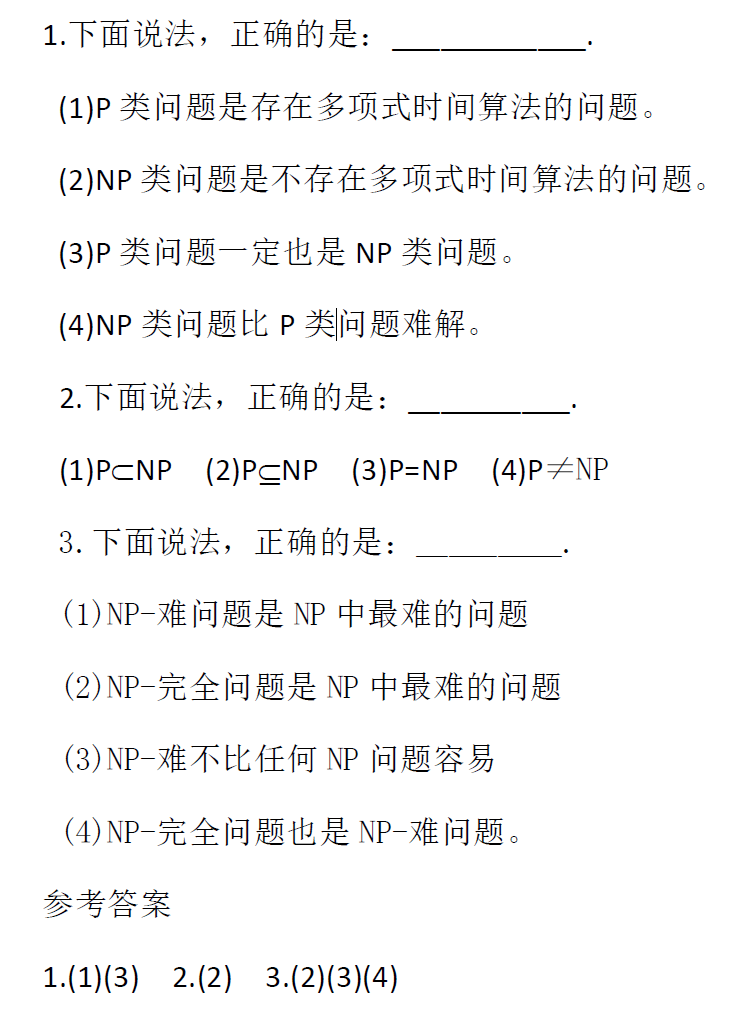
\includegraphics[width=0.7\textwidth]{images/title/补充练习.png}
		%\caption{解空间树搜索图}
		%\label{fig:解空间树搜索图}
	\end{figure}
\end{homeworkProblem}




% 引用文献
\bibliographystyle{unsrt}  % unsrt:根据引用顺序编号
\bibliography{refs}


\end{document}
